\section{coreOS:}
\label{sec:fleet}
CoreOS is a cluster-wide operating system to manage and run containers. It is a lightweight linux distribution which doesn't have any package manager. CoreOS uses docker containers to run its applications. It is platform independent which means coreOS can run on bare metal, virtual machine, cloud or cloud and physical machine together (coreOS website).

\begin{figure*}
\centering
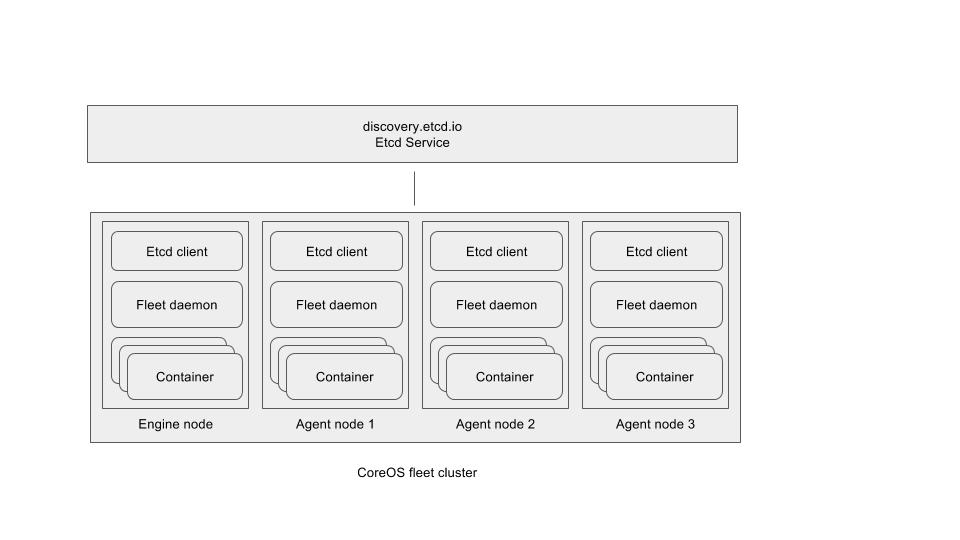
\includegraphics[scale=0.5]{./fig/fleet}
\caption{CoreOS Fleet Architecture}
\label{fig:fleetArch}
\end{figure*}

\begin{enumerate}
\item Fleet:
CoreOS's Fleet is the cluster manager which is built on systemd. Systemd, an init system, is a project separate than CoreOS which resolves the issues with sysV init and allows process management during boot-up. While systemd is for single machine, coreOS's Fleet is for the whole cluster. Fleet uses systemd unit files extended with some additional Fleet parameters to run any task. The systemd unit file are the configuration files which has the information about the task which Fleet uses to decide where to run the task. Fleet extends systemd feature to start, stop and monitor the units. Fleet can run two types of units: One is standard unit and other is global unit. Standard units are the tasks that run on a single node and it can be rescheduled on a new node if the node dies. Global units are the tasks that keep running cluster-wide i.e. on all the nodes. Global units are mainly used for services.
CoreOS has one fleet daemon running on each of the nodes on the cluster. Once the cluster is up, one of these fleet daemon is chosen as the master called engine and rest of the daemons are called agents. The engine daemon schedules the tasks dynamically monitoring the changes in the cluster. Engine process identifies the nodes to run the units and then forwards the tasks to that identified node to process it. This is done by agent process which keeps running on each of the nodes. The agent daemon keeps updating the status of the task back to the engine daemon. 

Following are the features of Fleet:

\item Etcd:
Etcd is a service that runs on every nodes. Its instance running on every machine needs to be synchronized and connected to build a cluster. Its job is more than just to coordinate between engine and agents daemons. It is used to store the key/value data for the whole cluster. It contains all the information about units, continuous updates about their states, configuration and nodes. Etcd is a stored in distributed manner over the cluster which makes it safe from the single node failure. 

\item Fault Tolerance:
The communication between engine and agents are done by using etcd tool. If any of the node fails while running the task, the agent daemon fails to update the status back to the engine. The engine understands that the node has failed and it reschedules the task on a new node. This self healing architecture of Fleet provides fault tolerance for each of the node. 

\item High Availability:
Fleet allows to run multiple instances of services on different nodes making it highly available.

\item Service Discovery:
Since the Etcd is distributed, any change in configuration doesn't need to be updated at each of the nodes individually. The change is updated on the nodes automatically. Etcd is also used for service discovery. CoreOS provides web URL for discovery service to connect instances of etcd running on different nodes. This web URL stores node addresses, metadata and the cluster size. 

\item Upgrades:
CoreOS uses Omaha protocol for latest updates. Instead of updating package by package, CoreOS is updated as a whole making it an atomic process. It uses dual partitioning technique which allows to rollback in case of failure. Since CoreOS is lightweight, executing an update and booting up is very fast.

\end{enumerate}